% coding:utf-8

%FOSAET, a LaTeX-Code for a electrical summary of basic electronics
%Copyright (C) 2013, Daniel Winz, Ervin Mazlagic

%This program is free software; you can redistribute it and/or
%modify it under the terms of the GNU General Public License
%as published by the Free Software Foundation; either version 2
%of the License, or (at your option) any later version.

%This program is distributed in the hope that it will be useful,
%but WITHOUT ANY WARRANTY; without even the implied warranty of
%MERCHANTABILITY or FITNESS FOR A PARTICULAR PURPOSE.  See the
%GNU General Public License for more details.
%----------------------------------------

\newpage
\section{Bipolartransistor}

\subsection{Eingangskennlinie}
\[ r_{BE} = \frac{\Delta U_{BE}}{\Delta I_B} \]

\subsection{DC Grosssignalverhalten}
\[ I_C \approx I_S \cdot e^{\frac{U_{BE}}{U_T}}\]
\[ U_T= \frac{k \cdot T}{q_0} \]
\[ U_T~(25^\circ C) = 25.8 mV \]
\begin{tabular}{@{}ll}
  $I_s$:        & Sättigungsstrom \\
  $U_T$:	    & "Temperaturspannung" \\
  $k$:          & Bolzmann-Konstante, $k=1.38 \cdot 10^{-23} [\frac{J}{K}]$ \\
  $T$:          & absolute Temperatur ($^\circ$C + 273,16 K) \\
  $q0$:         & Elementarladung = 1.602E-19As \\
\end{tabular}

\subsection{Stromverstärkung}
\[ B = \frac{I_C}{I_B} \]
\[ \beta = \frac{\Delta I_C}{\Delta I_B} \]

\subsection{Ausgangskennlinie}
\[ I_C \approx I_S \cdot e^{\frac{U_{BE}}{U_T}} \cdot 
\left(1 + \frac{U_{CE}}{U_A}\right) \]
\[ r_{CE} = \frac{\Delta U_{CE}}{\Delta I_C} \]
\[ D = \frac{\Delta U_{BE}}{\Delta U_{CE}} \]
\begin{tabular}{@{}ll}
  $U_A$:	    & Early-Spannung \\
  $D$:	        & differenzieller Rückwirkungsfaktor \\
\end{tabular}

\subsection{Modell gesteuerte Stromquelle}
\[ I_C(U_{BE}, T) = \frac{B \cdot I_S}{1 + B} 
\cdot \left(e^{\frac{U_{BE}}{n \cdot U_T}} - 1\right) 
\approx I_S \cdot e^{\frac{U_{BE}}{n \cdot U_T}} \]
\begin{tabular}{@{}ll}
  $I_S$:	    & Sättigungsstrom \\
  $n$:	        & Idealitätsfaktor $n = 1..2$ ($n = 1$ typisch) \\
\end{tabular}

\subsection{Emitterschaltung}
\begin{figure}[h!]
	\centering
	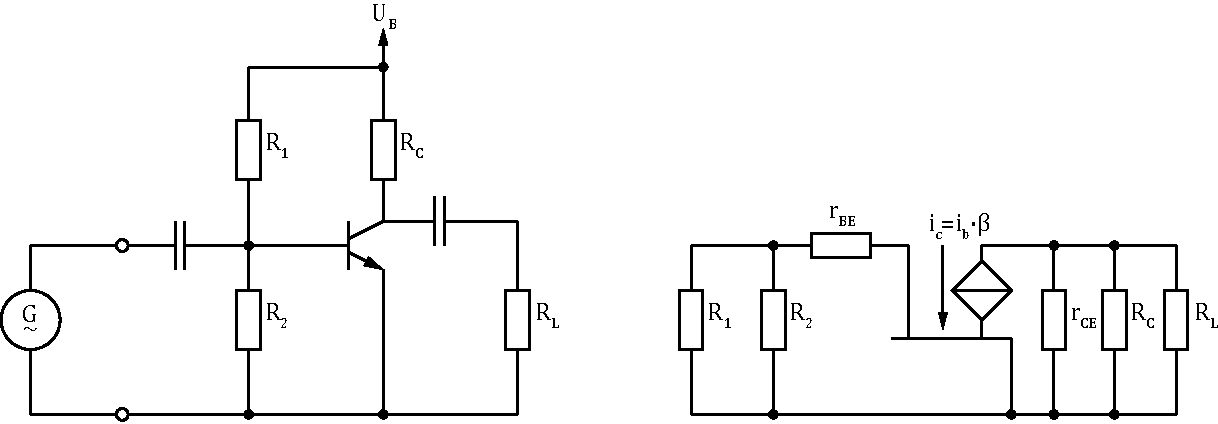
\includegraphics[width = \linewidth]{trans_emitter.pdf}
	\caption{Emitterschaltung mit Kleinsignalersatzschaltbild}
	\label{trans:emitterschaltung}
\end{figure}
\noindent
Spannungsverstärkung:
\[
	V_u = \frac{u_a}{u_e} = \beta \frac{r_{CE} \parallel R_C \parallel R_L}{r_{BE}}
\]
Eingangswiderstand:
\[
	r_e = r_{BE} \parallel R_1 \parallel R_2
\]
Stromverstärkung:
\[
	V_i = \frac{i_a}{i_e} = \beta \frac{r_{CE} \parallel R_C \parallel R_L}{R_L}
\]
Ausgangswiderstand:
\[
	r_a = r_{CE} \parallel R_C
\]

\newpage
\subsection{Emitterschaltung mit Stromgegenkopplung}
\begin{figure}[h!]
	\centering
	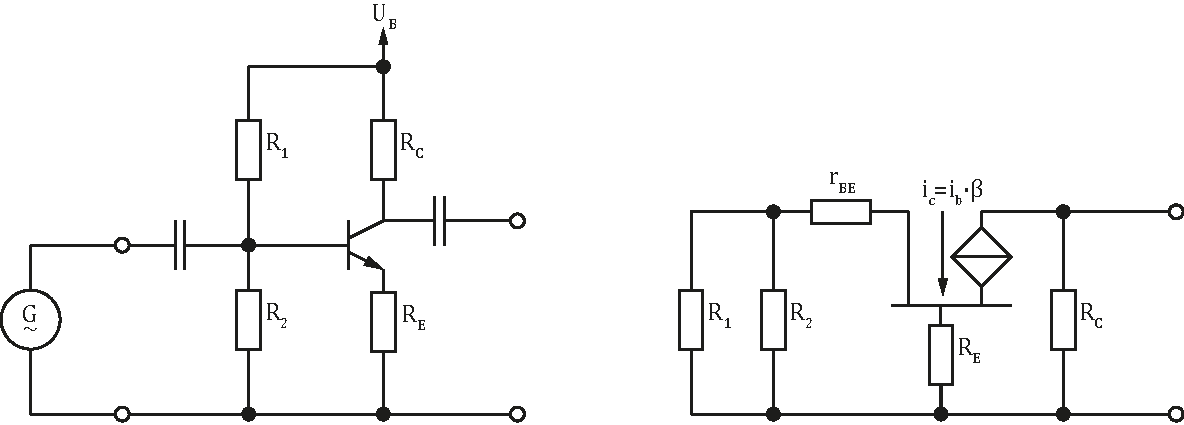
\includegraphics[width = \linewidth]{trans_emitter_stromgegen.pdf}
	\caption{Emitterschaltung mit Stromgegenkopplung und Kleinsignalersatzschaltbild}
	\label{trans:emitterschaltung_sgk}
\end{figure}
\noindent
Kleinsignal Formeln (Näherungen, $r_{CE} = \infty$):
\\\\
Spannungsverstärkung:
\[
	V_U = \frac{u_a}{u_e} = \frac{-\beta \cdot (R_C || R_L)}{r_{BE} + (1 + \beta) \cdot R_E} \stackrel{R_L \to \infty}{=} \frac{-\beta \cdot R_C}{r_{BE} + (1 + \beta) \cdot R_E} \approx \frac{-R_C}{R_E}
\]
Eingangswiderstand Transistor:
\[
	r_{eTr} \approx r_{BE} + (\beta + 1) \cdot R_E
\]
Gesamt Eingangswiderstand:
\[
	r_e \approx r_{eTr} \parallel R_1 \parallel R_2
\]
Ausgangswiderstand:
\[
	r_a \approx R_C
\]

\subsection{Emitterschaltung mit Transistorkapazitäten}
\[
	f_{go} = \frac{1}{2\pi \cdot R_q \parallel R_{eTR} \cdot C_{inT}}
\]
\[
	C_{inT} = C_{CB} \cdot (1-V_{ue}) + C_{BE} \cdot (1-V_{uc})
\]
\begin{tabular}{@{}ll}
  $V_{ue}$:	    & Verstärkung der Emitterschaltung ($\frac{U_{C}}{U_{B}}$) \\
  $V_{uc}$:	    & Verstärkung der Kollektorschaltung ($\frac{U_{E}}{U_{B}}$) \\
\end{tabular}

\subsection{Kollektorschaltung}
\begin{figure}[h!]
	\centering
	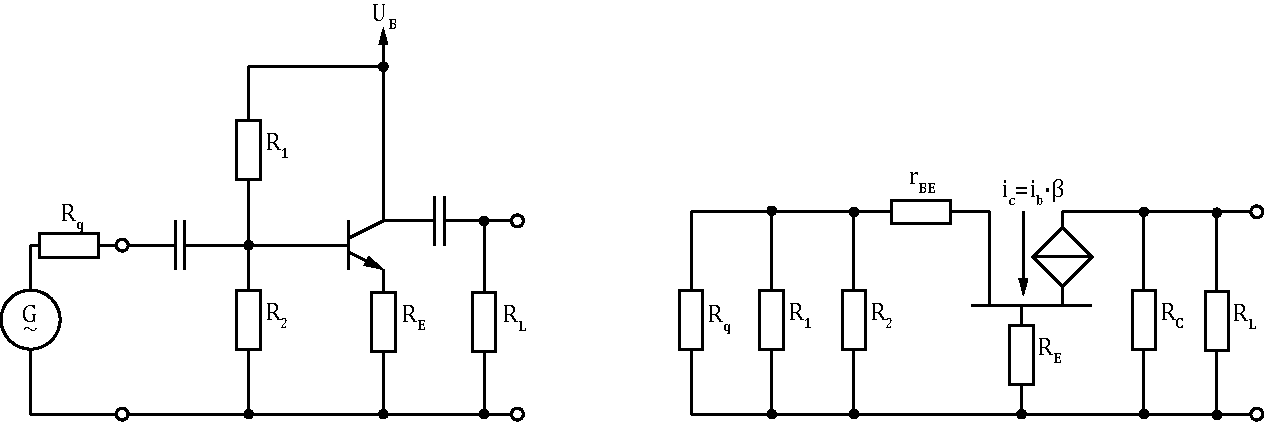
\includegraphics[width = \linewidth]{trans_kollektor.pdf}
	\caption{Kollektorschaltung mit Kleinsignalersatzschaltbild}
	\label{trans:kollektroschaltung}
\end{figure}
\noindent
Verstärkung:
\[
	V_U = \frac{u_a}{u_e} = \frac{1}{1 + \frac{r_{BE}}{(\beta + 1) \cdot R_E \parallel R_L}}
\]
Eingangswiderstand:
\[
	r_e = R_1 \parallel R_2 \parallel (r_{BE} + (\beta+1) \cdot R_E \parallel R_L)
\]
Ausgangswiderstand:
\[
	r_a = R_E \parallel \frac{R_1 \parallel R_2 \parallel R_q + r_{BE}}{\beta + 1}
\]

\newpage
\subsection{Darlingtonschaltung}
\begin{figure}[h!]
	\centering
	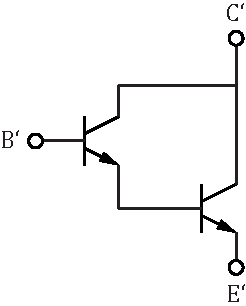
\includegraphics[scale = 0.6]{darlington.pdf}
	\caption{Darlingtonschaltung}
	\label{trans:darlington}
\end{figure}
\noindent
Ersatzkennwerte:
\[ \beta' = \beta_1 \cdot \beta_2 \]
\[ r_{BE}' = 2r_{BE1} \]
\[ r_{CE}' = \frac{2}{3} r_{CE2} \]

\subsection{Komplementär Darlington-Schaltung}
\begin{figure}[h!]
	\centering
	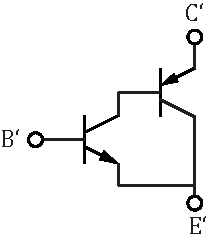
\includegraphics[scale = 0.6]{darlington_komp.pdf}
	\caption{Komplementär Darlington-Schaltung}
	\label{trans:darlington_komp}
\end{figure}
\noindent
Ersatzkennwerte:
\[ \beta' = \beta_1 \cdot \beta_2 \]
\[ r_{BE}' = r_{BE1} \]
\[ r_{CE}' = \frac{1}{2} r_{CE2} \]